\chapter{Funkcja kosztu}
\thispagestyle{chapterBeginStyle}

\section{Ogólny opis}
W kontekście konstruowania modelu predykcyjnego, funkcja kosztu $L$, to funkcja, która pozwala na ocenę skuteczności predykcji modelu. W tej pracy utrzymana jest konwencja minimalizowania funkcji kosztu, to znaczy, że poszukiwany jest model posiadający najmniejszą średnią wartość funkcji kosztu na ustalonym zbiorze testowym. Zadaniem funkcji kosztu jest przedstawienie skuteczności predykcji za pomocą jednej liczby w taki sposób, że proces minimalizowania wartości funkcji kosztu będzie w pewnym sensie polepszał jakość predykcji (usprawniał model). Podstawowym problemem podczas konstruowania modelu jest wybór funkcji kosztu. W tej pracy funkcją kosztu jest zaproponowana przez firmę \texttt{Lyft} funkcja $L$ opisana poniżej.

\section{Równanie funkcji kosztu}

\noindent
Załóżmy, że pozycje wyjściowe są równe:

\begin{equation}
V_{t} = [(x_{0},y_{0}), (x_{1},y_{1}), ... , (x_{49},y_{49})]
\end{equation}

\noindent
Model przewiduje trzy trajektorie i prawdopodobieństwa ($k \in \{0, 1, 2\}$):

\begin{equation}
\hat{V}_{t}^{k} = [(\hat{x}_{0}^{k},\hat{y}_{0}^{k}), (\hat{x}_{1}^{k},\hat{y}_{1}^{k}), ... , (\hat{x}_{49}^{k},\hat{y}_{49}^{k})]
\end{equation}

\begin{equation}
\hat{P}_{t}^{k} = P(\text{\upshape trajektoria}\:\hat{V}_{t}^{k}\:\text{\upshape zostanie zrealizowana})
\end{equation}

\noindent
Załóżmy, że pozycje zawarte w $V_{t}$ oraz $\hat{V}_{t}^{k}$ dotyczą chwil:

\begin{equation}
[t+0.1, t+0.2, ... , t+5.0]
\end{equation}

\noindent
Załóżmy, że pozycje wyjściowe są modelowane przez mieszaninę niezależnych wielowymiarowych rozkładów normalnych. Przy takich założeniach funkcja wiarygodności (ang. likelihood) ma postać:

\begin{equation}
p(V_{t}|\hat{P}_{t}^{0,1,2}, \hat{V}_{t}^{0,1,2}) = p(x_{0,...,49},
y_{0,...,49}|\hat{P}_{t}^{0,1,2}, \hat{V}_{t}^{0,1,2}) =
\end{equation}

\begin{equation}
= \sum_{k}\hat{P}_{t}^{k}\cdot\mathcal{N}(x_{0,...,49}|\hat{x}_{0,...,49}^{k}, \Sigma=1)\cdot\mathcal{N}(y_{0,...,49}|\hat{y}_{0,...,49}^{k}, \Sigma=1) =
\end{equation}

\begin{equation}
= \sum_{k}\hat{P}_{t}^{k}\cdot\prod_{j=0}^{j=49}\mathcal{N}(x_{j}|\mu=\hat{x}_{j}^{k}, \sigma=1)\cdot\mathcal{N}(y_{j}|\mu=\hat{y}_{j}^{k}, \sigma=1)
\end{equation}

\noindent
Tak otrzymaną funkcję wiarygodności (ang. likelihood) możemy następnie przekształcić do funkcji kosztu \texttt{NLL} (ang. negative log-likelihood):

\begin{equation}
L = -ln(p(V_{t}|\hat{P}_{t}^{0,1,2}, \hat{V}_{t}^{0,1,2})) =
\end{equation}

\begin{equation}
= -ln(\sum_{k}\hat{P}_{t}^{k}\cdot e^{-\frac{1}{2}\sum_{j=0}^{j=49}(x_{j}-\hat{x}_{j}^{k})^{2}+(y_{j}-\hat{y}_{j}^{k})^{2}}) =
\end{equation}

\newpage

\section{Wizualizacja funkcji kosztu}

\begin{figure}[H]
    \centering
    \subfloat[Wyjściowe pozycje agenta EGO]{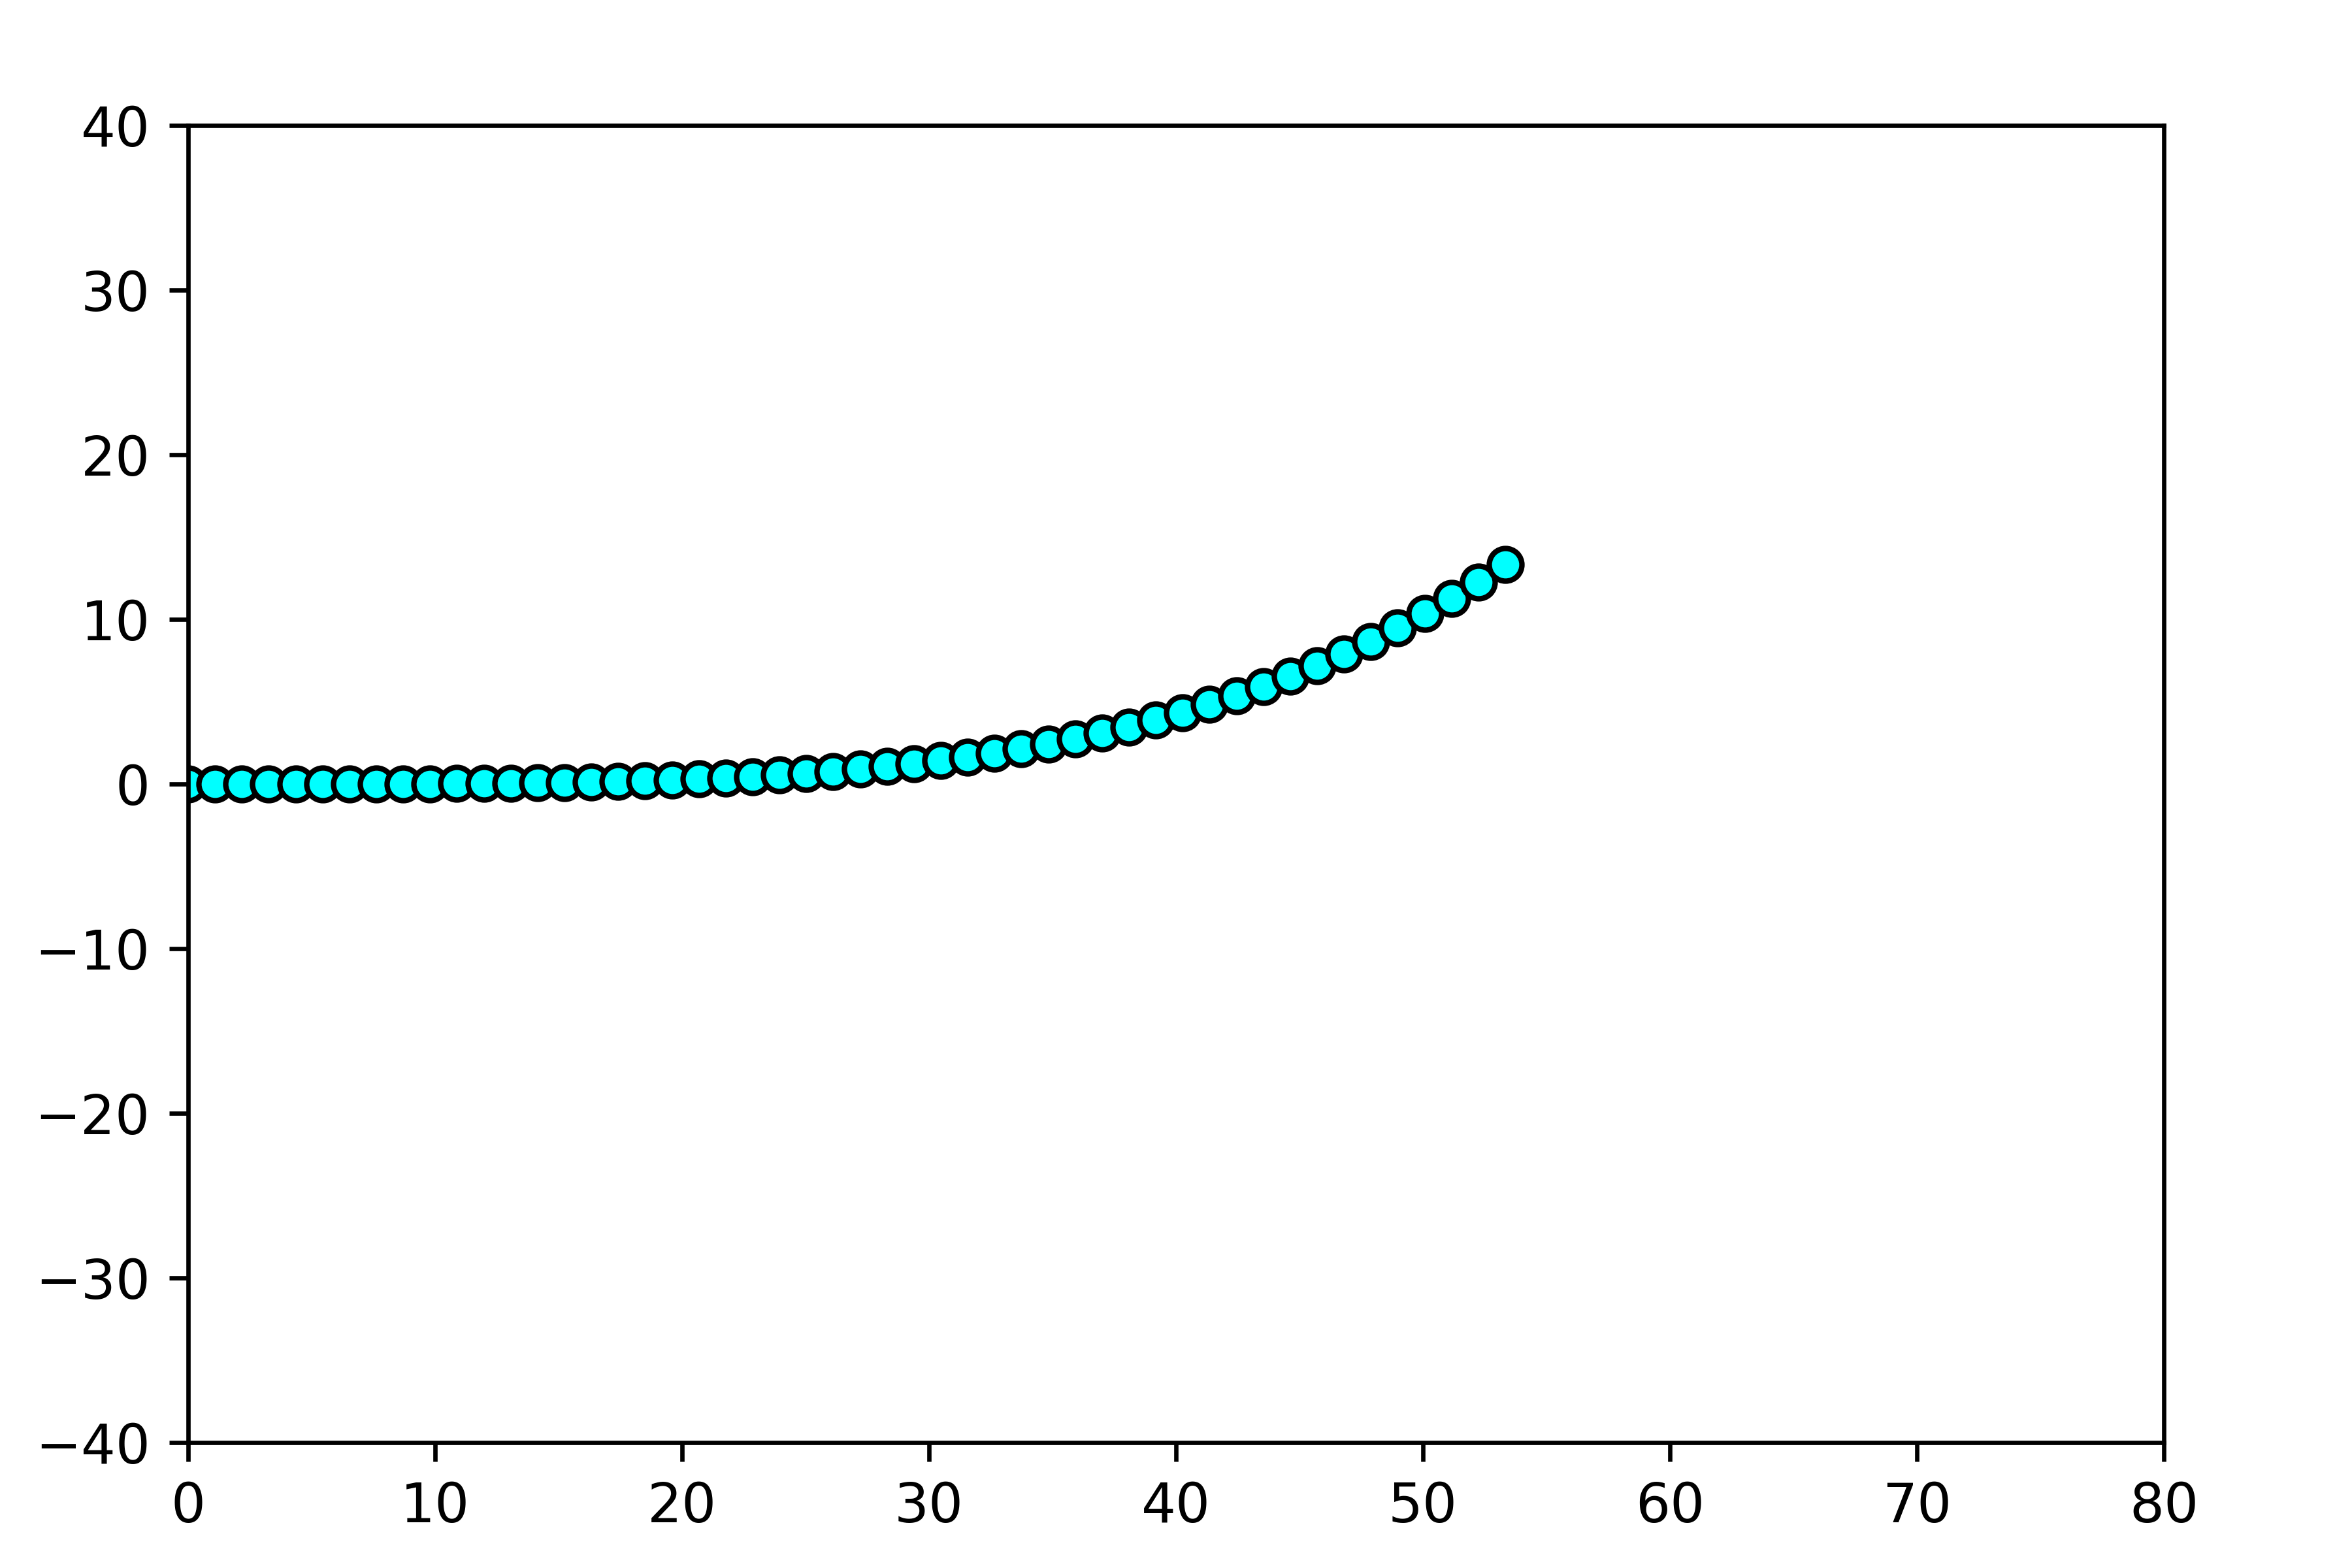
\includegraphics[width=0.5\textwidth]{loss0.png}}
    \subfloat[Trajektorie naśladujące predykcje modelu]{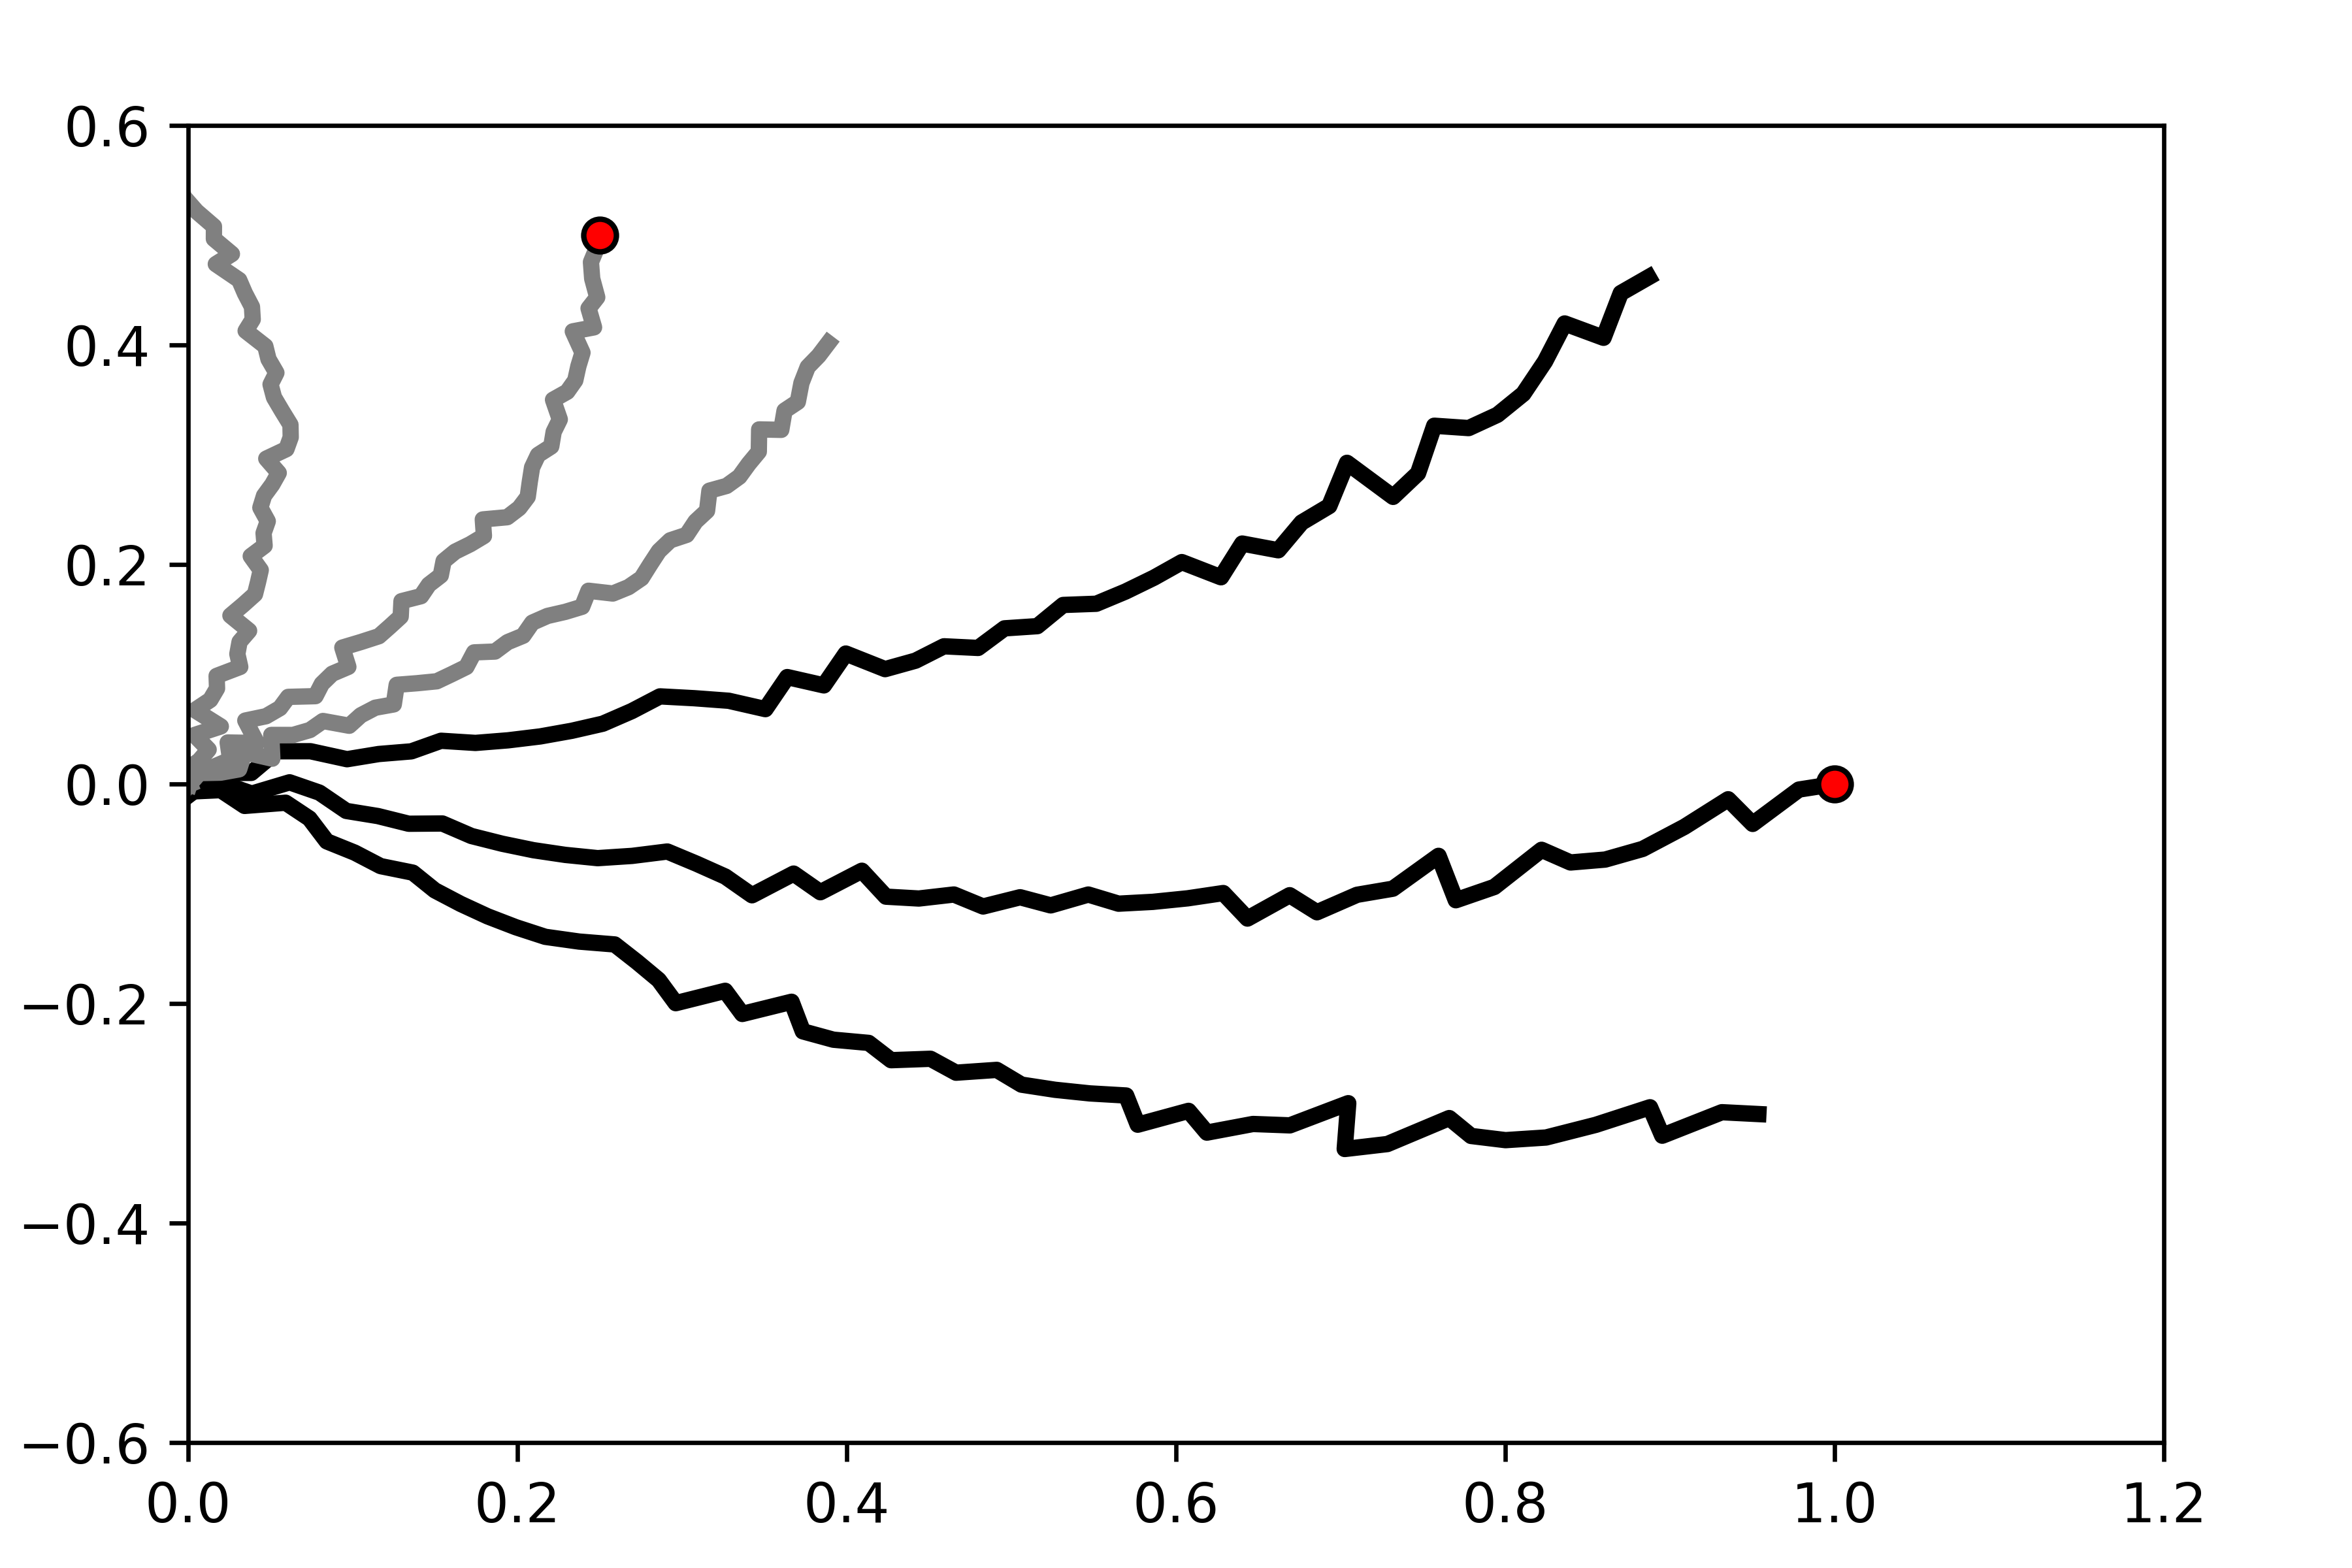
\includegraphics[width=0.5\textwidth]{loss1.png}}
\end{figure}

\begin{figure}[H]
    \centering
    \subfloat[Wartości funkcji kosztu]{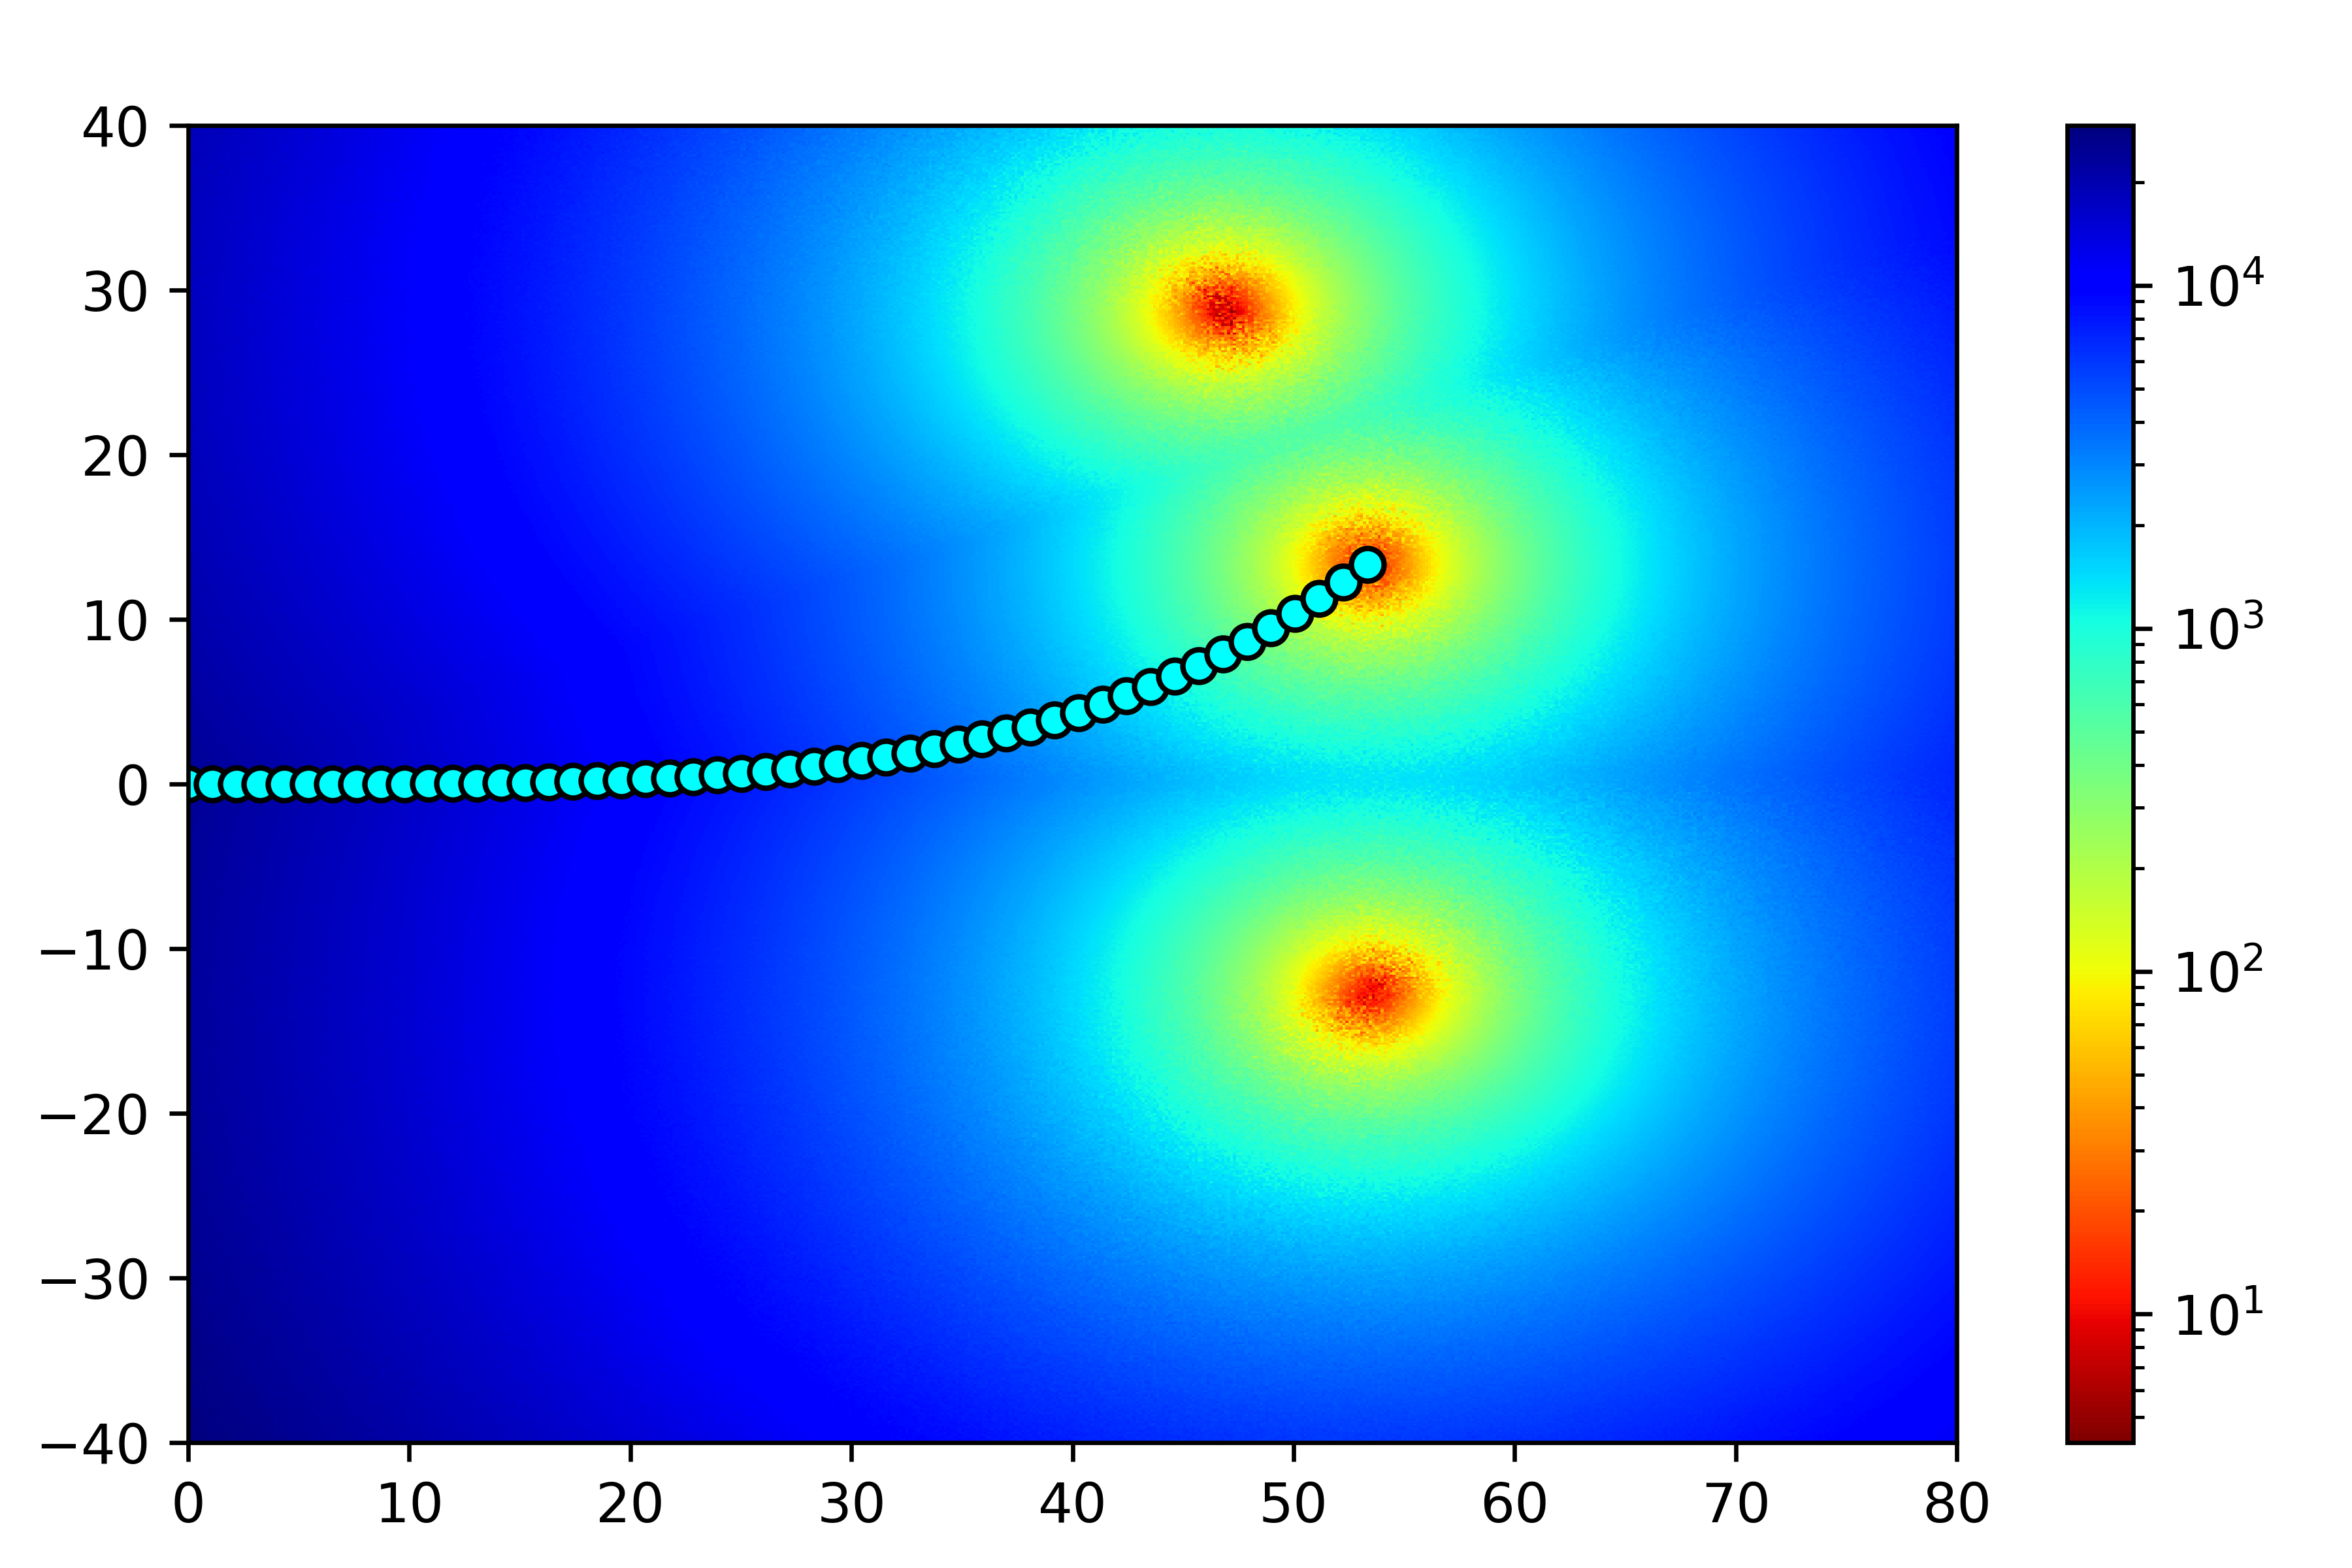
\includegraphics[width=0.5\textwidth]{loss2.png}}
    \subfloat[Pierwsze minimum lokalne]{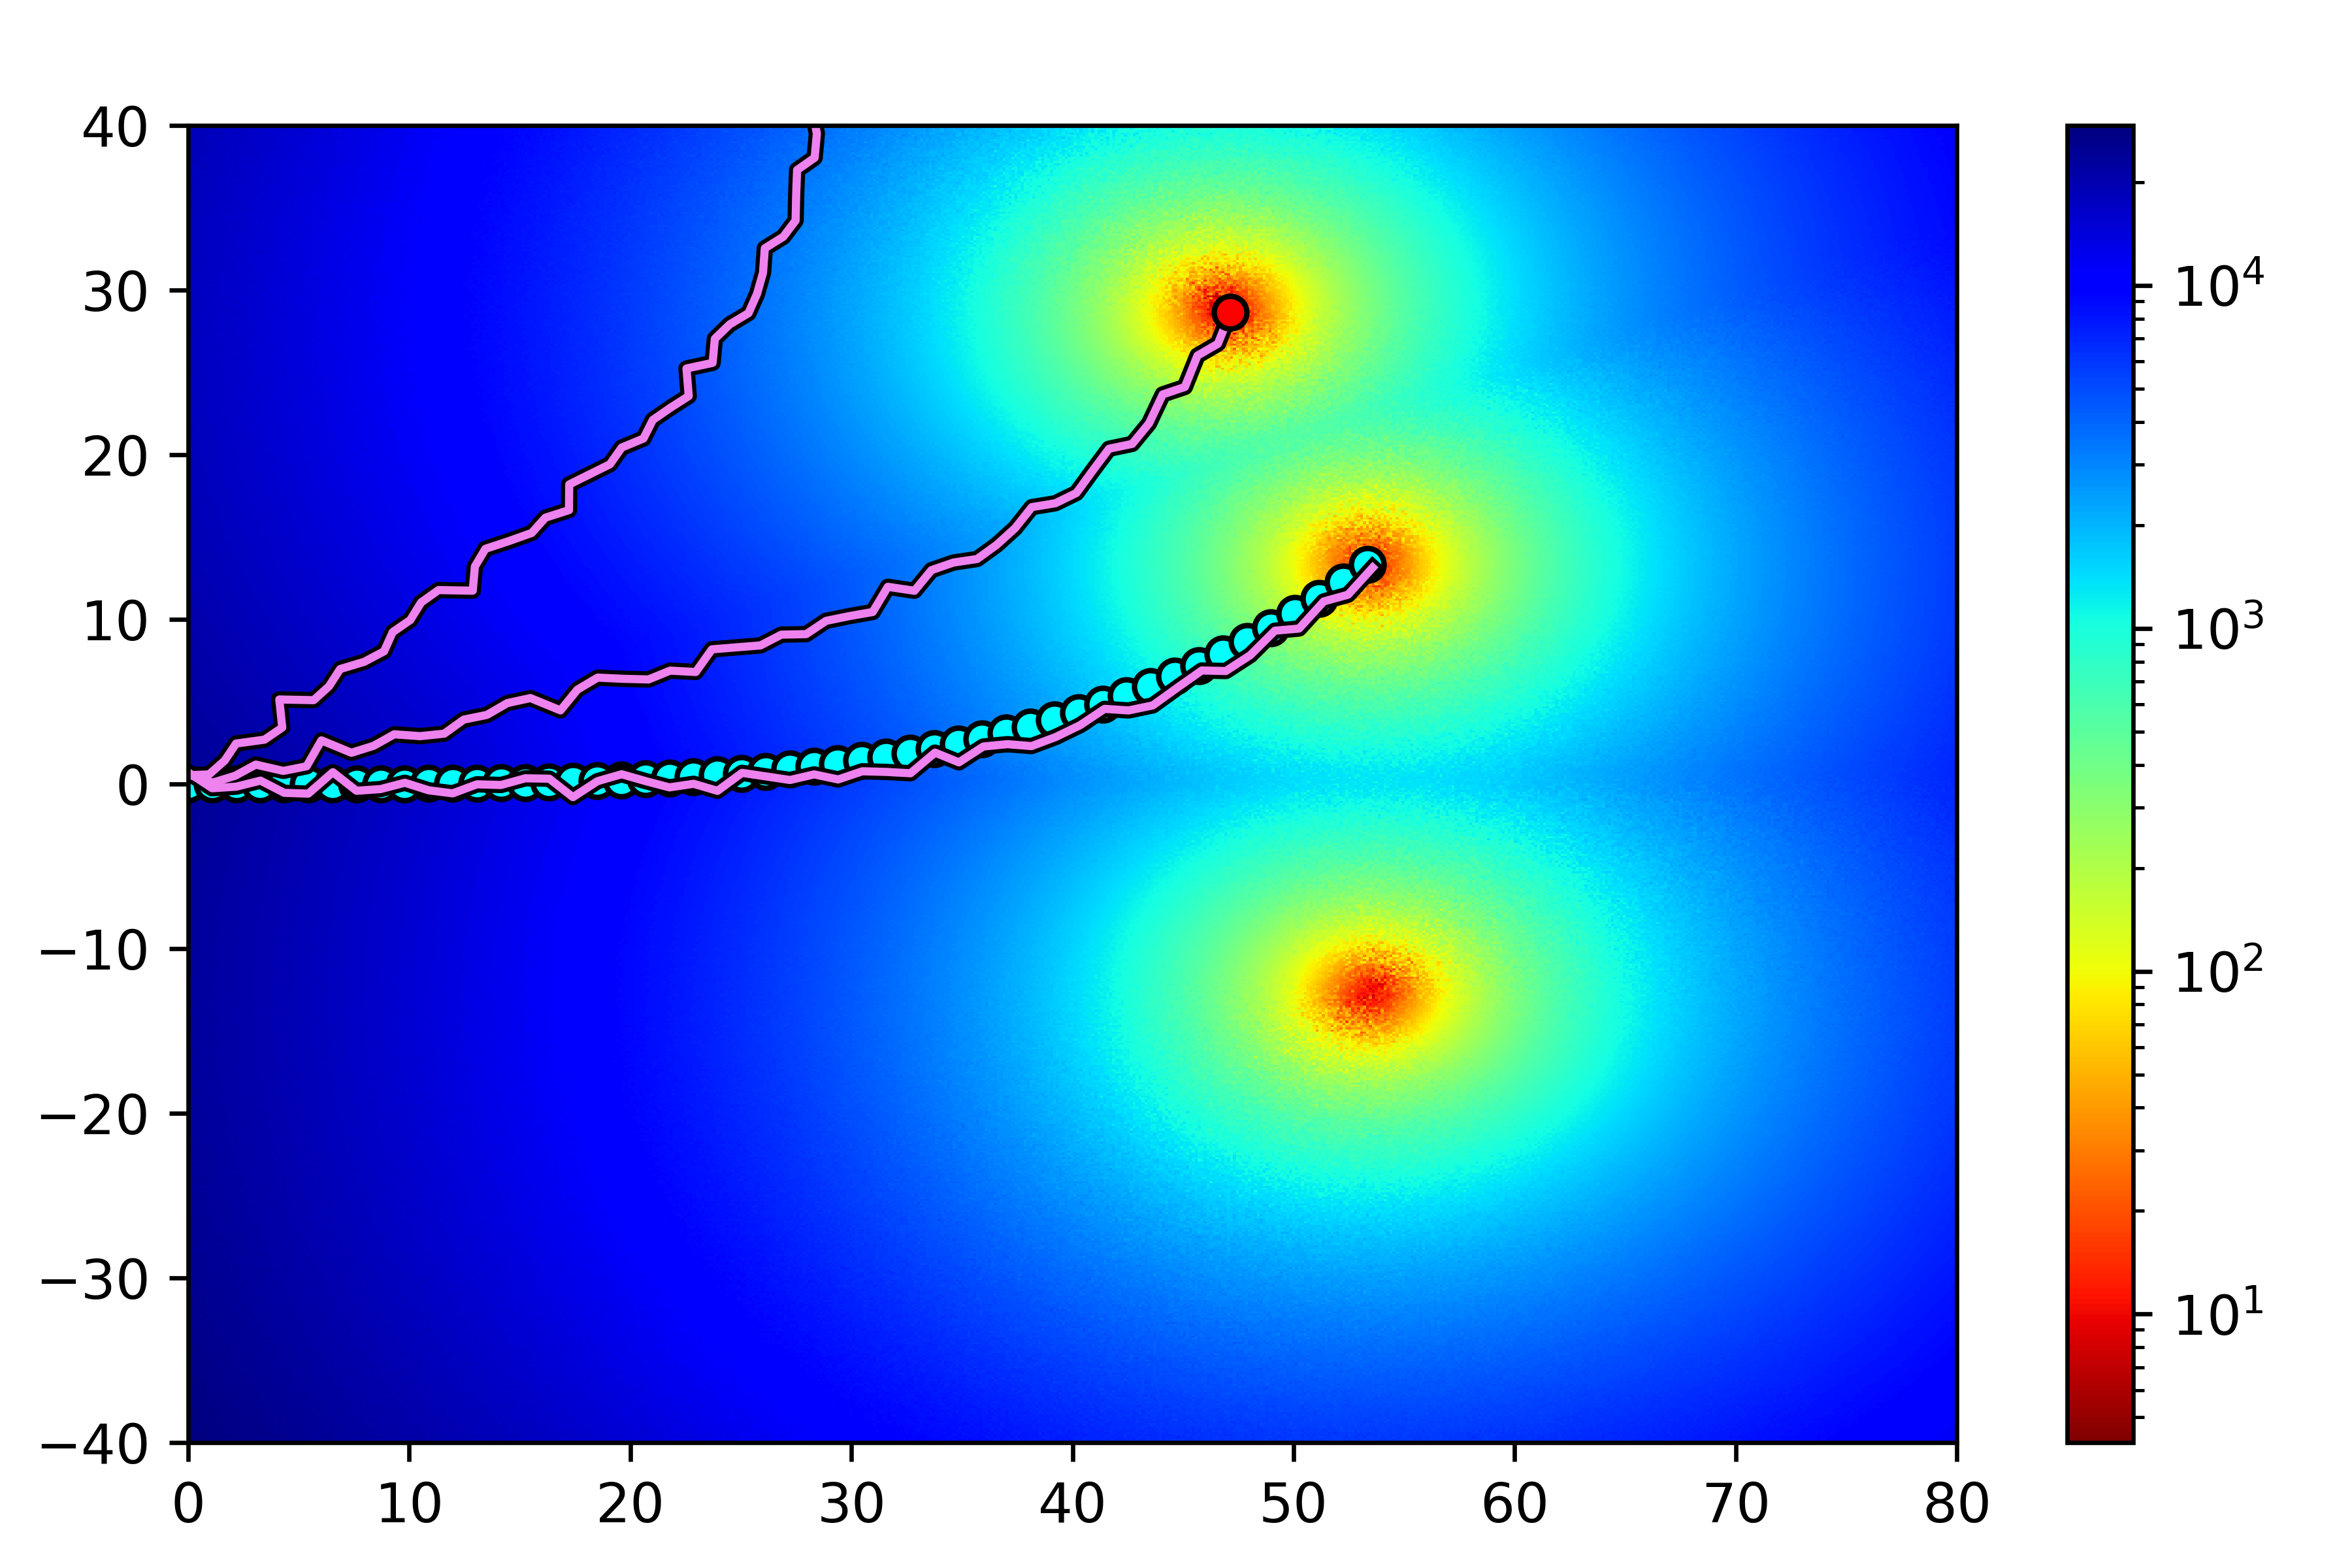
\includegraphics[width=0.5\textwidth]{loss3.png}}
\end{figure}

\begin{figure}[H]
    \centering
    \subfloat[Drugie minimum lokalne]{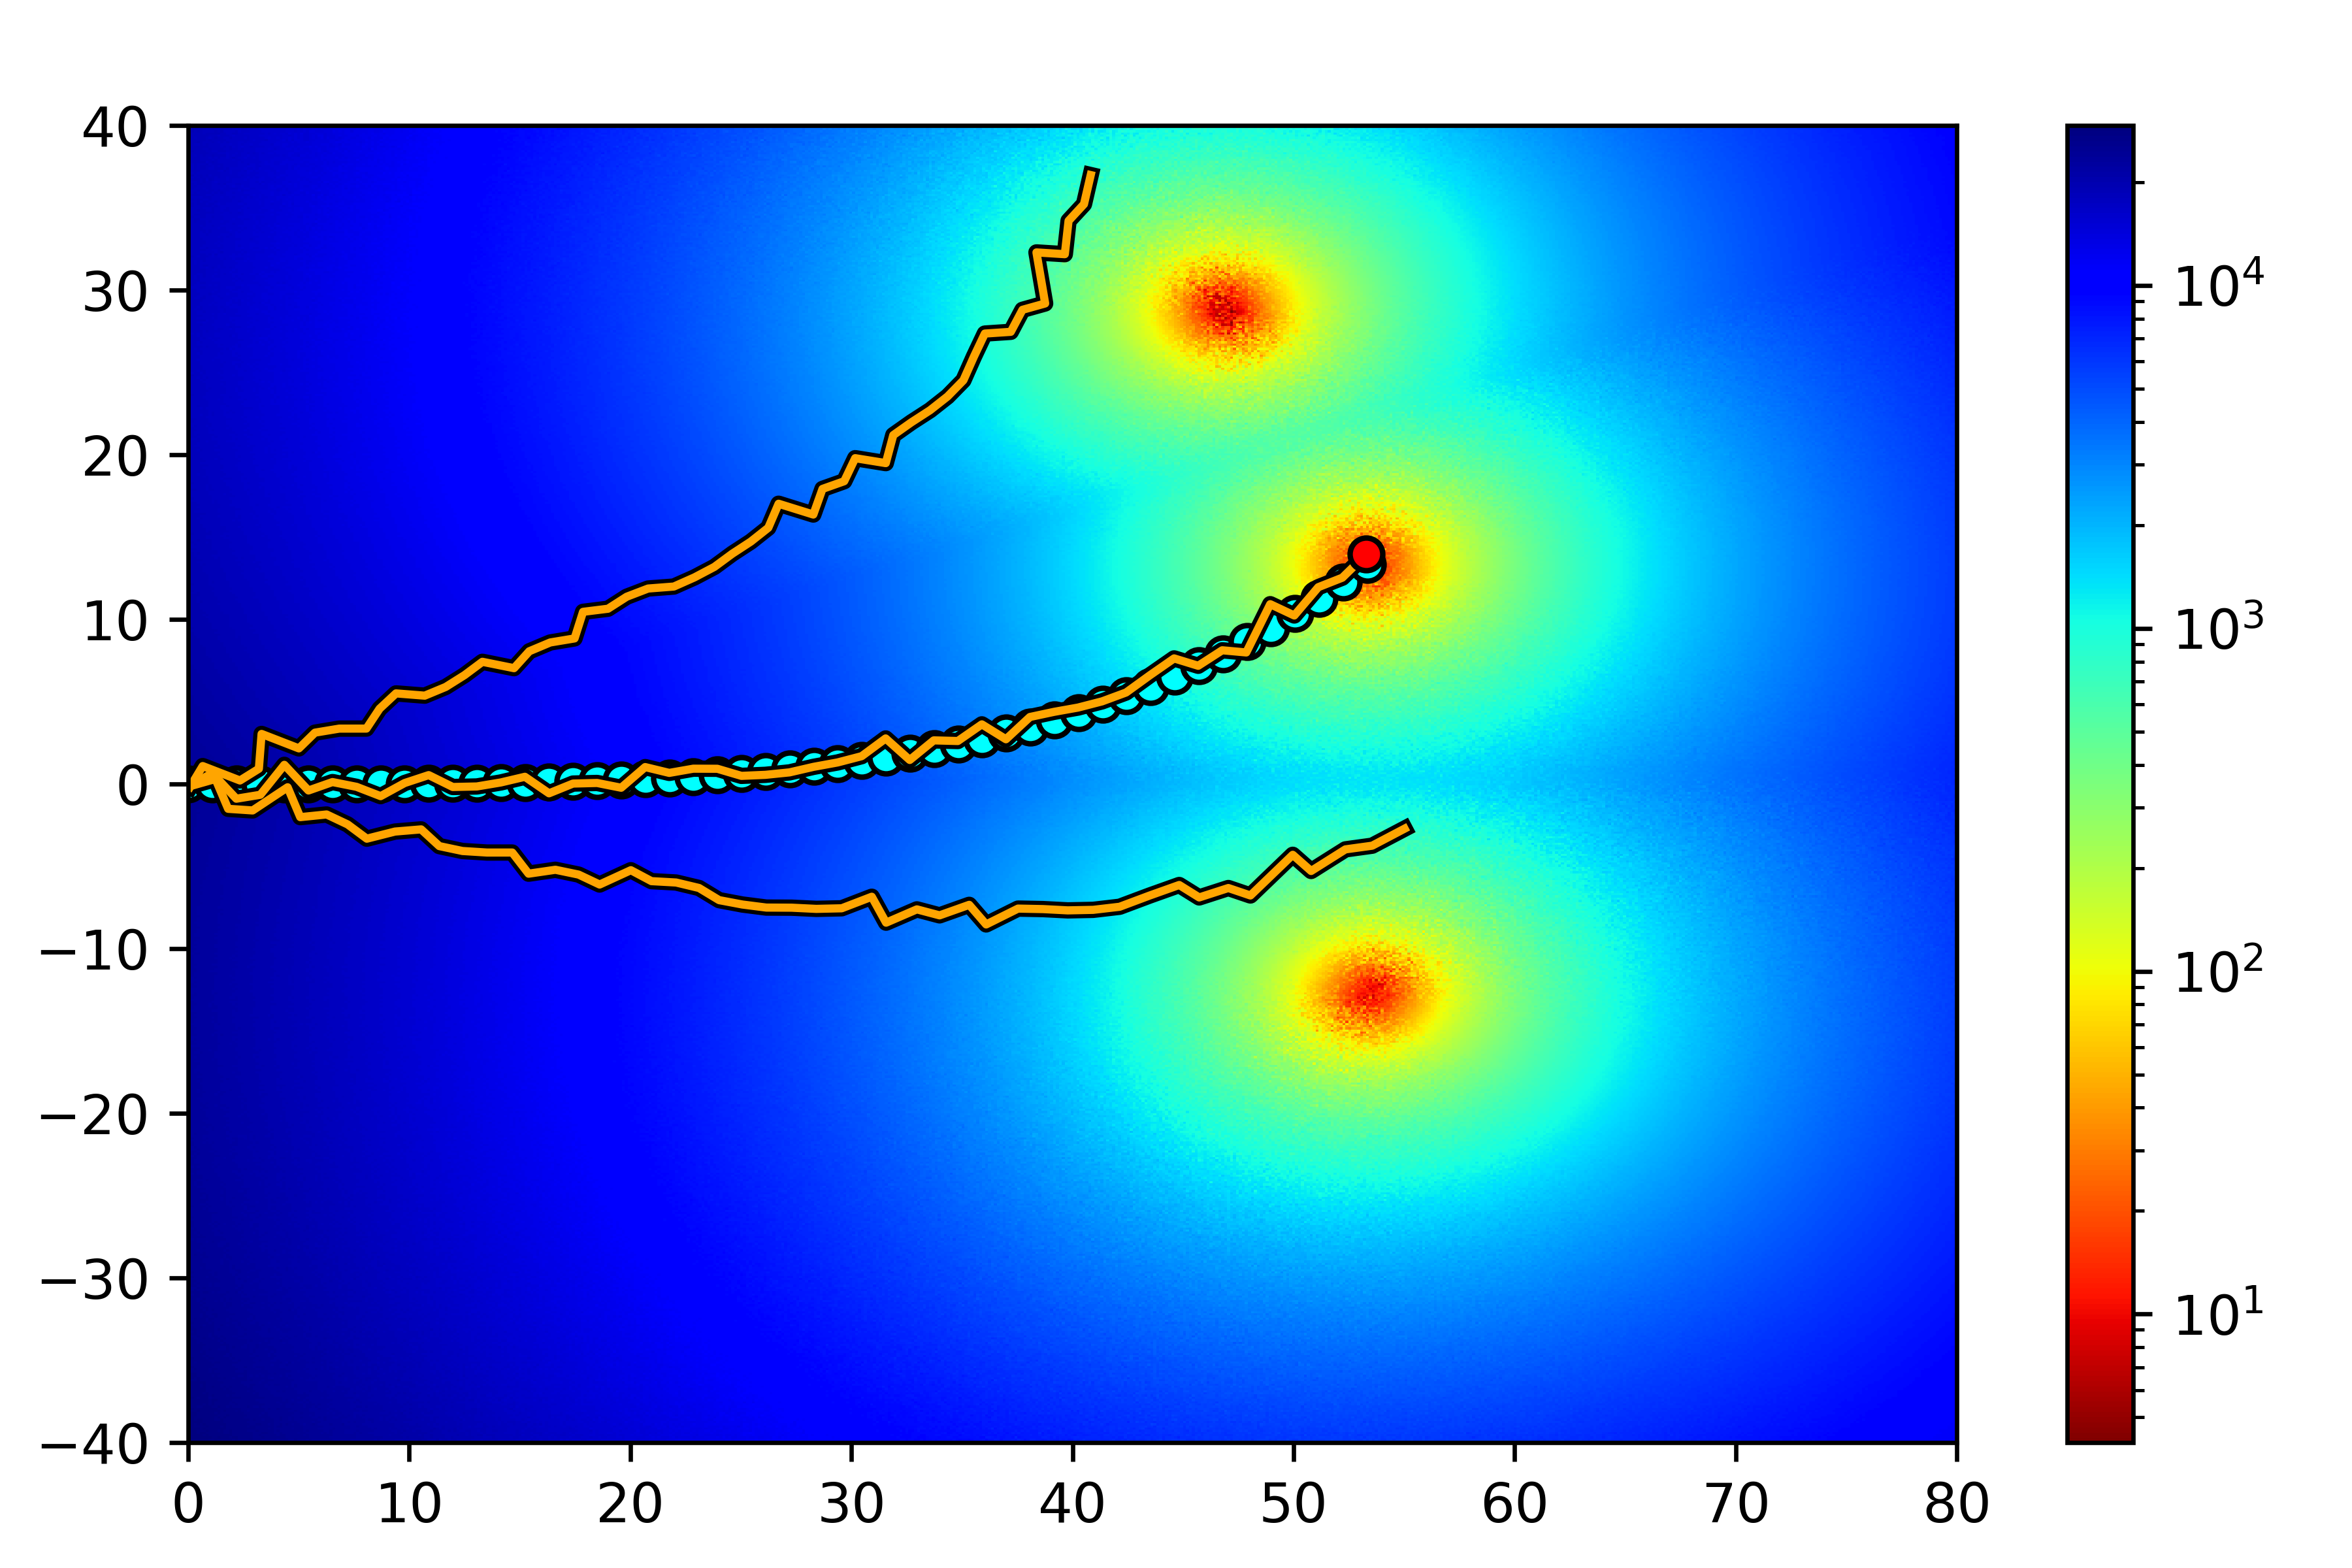
\includegraphics[width=0.5\textwidth]{loss5.png}}
    \subfloat[Trzecie minimum lokalne]{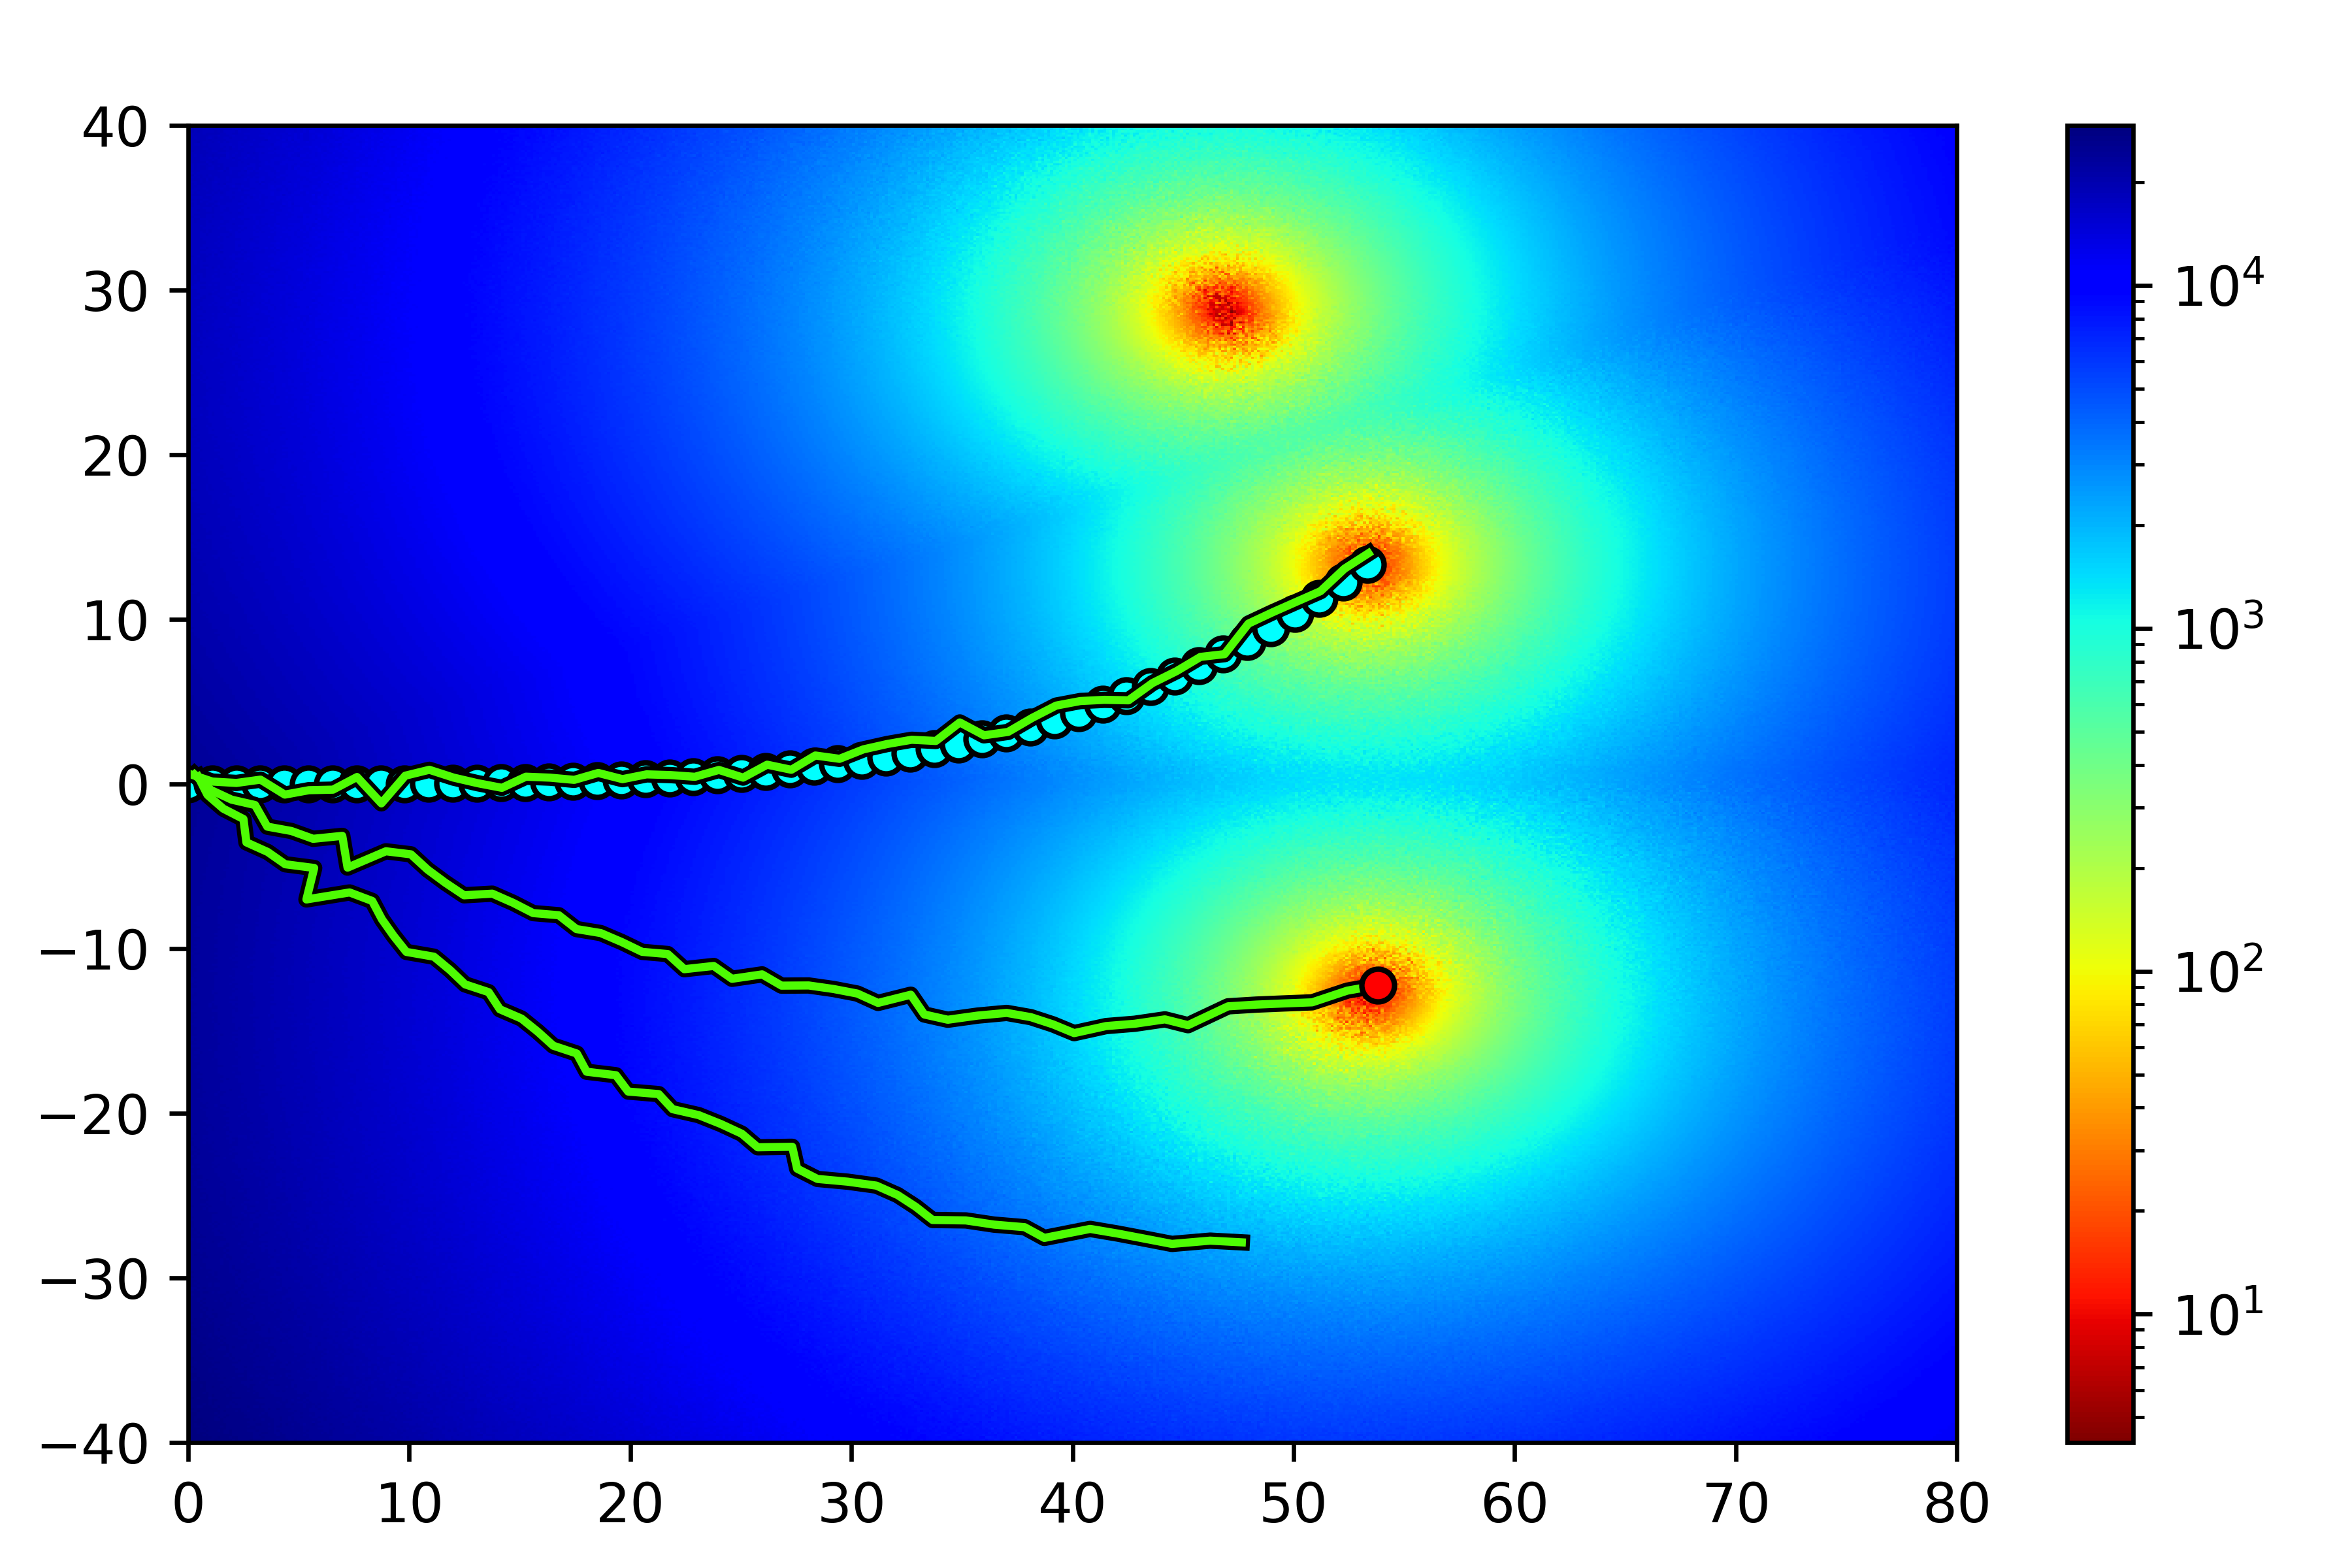
\includegraphics[width=0.5\textwidth]{loss4.png}}
\end{figure}

\newpage

\section{Opis wizualizacji}

\subsubsection{(a) Wyjściowe pozycje agenta EGO}
Na wykresie seledynowymi kropkami zaznaczono wyjściowe pozycje pewnego agenta \texttt{EGO} ze zbioru. Są to współrzędne, które nie są dostępne w chwili $t$, gdyż dotyczą następnych pięciu sekund. Przewidywanie tych współrzędnych jest zadaniem modelu predykcyjnego, który ma za zadanie zrobić to z jak największą dokładnością (ma możliwość przewidzenia trzech scenariuszy, czyli trzech trajektorii).
\subsubsection{(b) Trajektorie naśladujące predykcje modelu}
Na tym wykresie zaprezentowano pewne trzy trajektorie (uzależnione od parametru nazywanego \textit{punktem definującym trajektorie}), trajektorie te są z góry ustalone i mają za zadanie symulować działanie modelu predykcyjnego. Poniżej omówione zostanie jak trajektorie te wpływają na funkcję kosztu oraz to jak sprawić aby funkcja kosztu była jak najmniejsza. Zaproponowane trajektorie zaznaczone na czarno są uzależnione od punktu definującego trajektorie (tutaj ($x=1, y=0$)), który ustala położenie trzech trajektorii, poprzez obrót i skalowanie trajektorii bazowych (trzy czarne trajektorie). Na szaro zaznaczone zostały trajektorie bazowe obrócone i przeskalowane w wyniku zmiany położenia punktu definiującego trajektorie ($x=0.25, y=0.5$). Położenie punktu definiującego trajektorie i jego wpływ na funkcję kosztu będzie następnie analizowane za pomocą mapy ciepła (ang. heat map).
\subsubsection{(c) Wartości funkcji kosztu}
Na tym wykresie przedstawione zostały pozycje agenta \texttt{EGO} oraz mapa ciepła przedstawiająca wartość funkcji kosztu w zależności od pozycji punktu definiującego trajektorie, dla trajektorii bazowych zaproponowanych na wykresie (b). Na wykresie można zauważyć trzy minima lokalne.
\subsubsection{(d), (e), (f) Pierwsze, drugie i trzecie minimum lokalne}
Położenie minimów lokalnych, na wykresie (d), (e) i (f) nie jest przypadkowe. Minima lokalne odpowiadają takim położeniom punktu definiującego trajektorię, które sprawiają, że jedna z trajektorii pokrywa się z trajektoriami wyjściowymi agenta \texttt{EGO}. Aby uzyskać małą wartość funkcji kosztu przynajmniej jedna z trajektorii musi być zgodna z tą, która została zrealizowana (zgodna z pozycjami wyjściowymi). Gdy jedna z trzech przewidywanych trajektorii jest blisko wyjściowej trajektorii agenta \texttt{EGO}, powoduje to, że prawdopodobieństwo uzyskania obserwacji (trajektorii agenta \texttt{EGO}) z mieszaniny rozkładów normalnych, gdzie jedna z trajektorii jest blisko trajektorii agenta \texttt{EGO}, jest w pewnym sensie duże. Wtedy funkcja wiarygodności przyjmuje odpowiednio dużą wartość, a co za tym idzie funkcja kosztu odpowiednio małą wartość, gdyż na funkcję wiarygodności o odpowiednio dużej wartości jest nakładany logarytm (funkcja rosnąca) oraz ujemny znak (funkcja malejąca). Z powyższego wynika, że funkcja kosztu spełnia swoje zadanie, minimalizowanie jej w pewnym sensie zmusza model do przewidywania jednej z trzech trajektorii dostatecznie blisko pozycji wyjściowych agenta \texttt{EGO}. Można łatwo pokazać, że funkcja kosztu osiąga wartość najmniejszą równą 0 wtedy i tylko wtedy, gdy wszystkie trajektorie przewidywane przez model, które nie posiadają przewidywanego prawdopodobieństwa równego 0, dokładnie pokrywają się z pozycjami wyjściowymi agenta \texttt{EGO}.